\documentclass[manuscript,screen,nonacm]{acmart}
\usepackage{amsmath}
\usepackage{booktabs}
\usepackage{tabularx}
\usepackage{tikz}
\usetikzlibrary{arrows.meta,positioning}
\settopmatter{printacmref=false}
\setcitestyle{numbers,sort&compress}
\setcopyright{none}
\title{When Verification Helps: Failure Boundaries of Structural Remediation Decisions Under Imperfect Evidence}
\author{Ezekiel Ologunde}
% Country is intentionally blank; no geographic affiliation was supplied.
\affiliation[obeypunctuation=true]{\institution{Independent Researcher}\country{}}
\email{ologunde@bu.edu}
\authorsaddresses{Author's address: Ezekiel Ologunde, Independent Researcher; email: \href{mailto:ologunde@bu.edu}{ologunde@bu.edu}.}
\renewcommand{\shortauthors}{Ezekiel Ologunde}
\keywords{attack graphs, value of information, remediation, source dependence, reproducibility, negative results}
\begin{abstract}
Verification can improve a remediation decision, but it consumes resources that could otherwise fund intervention. Its value also depends on the probability model used to interpret observations. We study these boundaries with an exact, finite structural-exposure benchmark and a separate public-package evidence audit. A frozen grid crosses three four-gate graphs, two joint priors, eight evidence patterns, and two verification costs, producing 96 cases and 960 policy evaluations. A policy using reported source groups and observation age improves on its immediate-action counterpart in 27 cases, ties in 69, and worsens in none. Its mean-loss advantage over naive verification is only 0.00025, so the results do not establish broad provenance-aware superiority. An independence approximation makes verification harmful in two constructed cases, increasing expected loss from 2.60 to 2.78. A universal-cut control and a patch-affordability threshold explain large groups of ties. Independent rational-arithmetic scoring reproduces the saved decisions' outcomes to floating-point precision. A deterministic sample of 20 OSV PyPI advisory/package pairs all has explicit GitHub source attribution, an expected consequence of the sampling rule rather than independent corroboration. Isolated package checks demonstrate the feasibility and limits of additional behavioral evidence. The contribution is a transparent characterization of failure and no-benefit conditions, with preserved setup failures and reproducible artifacts, not a new value-of-information algorithm or evidence of operational remediation effectiveness.
\end{abstract}
\begin{document}
\maketitle

\section{Introduction}
Security teams frequently decide whether to investigate a reported vulnerability or spend their available resources on remediation immediately. A report may be outdated, copied across databases, or attached to the wrong source group. Separately, multiple paths through a network may depend on a shared fact. These two forms of dependence concern different objects: the first concerns how evidence was produced, while the second concerns which paths are enabled. Treating either as independence can change a decision even when the underlying graph is unchanged.

Additional information is not automatically useful under a shared verification and intervention budget. A query can identify the correct action but leave too little budget to take it. Conversely, an affordable action may already disconnect every target, making further information irrelevant to the selected objective. A favorable comparison against immediate patching therefore does not, by itself, establish that sophisticated provenance handling caused the benefit. Ordinary value of information (VOI) may explain nearly all of it.

This paper examines these distinctions in a small model whose decisions and consequences can be enumerated exactly. Its empirical scope is intentionally bounded. The synthetic experiment measures weighted structural reachability, not observed attacker success, incident frequency, or monetary damage. A separate public evidence audit examines source attribution and whether selected affected/fixed package pairs permit isolated behavioral checks. It does not provide probability estimates for the synthetic model.

We ask two research questions. \textbf{RQ1:} Under specified graph and observation models, when does query-then-patch improve or worsen structural exposure relative to immediate patching? \textbf{RQ2:} Which source relationships and executable behavioral distinctions can be established for a fixed, transparently selected set of public package advisories?

The study contributes an inspectable finite benchmark, a paired analysis that separates ordinary verification gains from the small incremental effect of source and age handling, and a public-artifact feasibility audit with explicit exclusions. Two concrete counterexamples show harmful verification after dependence approximation. Negative controls explain when information has no decision value. A post hoc independent rational calculation checks the numerical results without changing the frozen planner. These contributions are methodological and descriptive. We make no claim to a new uncertainty formalism, an optimal scalable solver, discovery of previously unknown vulnerabilities, or field-wide priority for the combined setting.

\section{Related Work and Positioning}
Nguyen, Palani, and Nicol model uncertain network facts and correlations induced by shared indicators, and discuss information gathering and hardening in network-security analysis~\cite{nguyen}. Our shared gates and uncertainty-reduction motivation therefore extend established ideas. The distinction examined here is a particular experiment combining erroneous reported source groups, observation age, a noisy query, and a shared query/patch budget. A difference from one paper is not proof of a field-wide gap.

Costly observation selection and conditional plans are standard VOI problems. Krause and Guestrin provide algorithms and complexity results for graphical models~\cite{krause}. Our exhaustive one-query planner is a conventional baseline for a tiny state space. It is not a new VOI algorithm. Source dependence also predates this study: Dong, Berti-Equille, and Srivastava study truth discovery in the presence of copying~\cite{dong}. We do not infer copying from records. Instead, we supply source labels, deliberately corrupt some labels, and assess the resulting decisions.

Partially observable security games already support defense under uncertain observations. Khakpour and Parker synthesize defenses using one-sided partially observable games, with a sound transformation under stated restrictions~\cite{khakpour}. CyGATE includes patching, monitoring deployment, costs, and belief updates~\cite{cygate}. Combining sensing and patching is consequently not a defensible novelty claim. Our simpler static endpoint isolates particular budget and dependence effects; it does not compete with these systems on their dynamic objectives.

CAPG-v2 prioritizes patches through an impact-weighted attack-position model and finite-horizon attacker rollouts~\cite{capg}. Its endpoint incorporates action selection and attempts, whereas ours integrates reachability over latent graph states. The quantities cannot be compared numerically without a common model. We therefore do not present CAPG-v2 as a reproduced baseline or claim that it ignores evidence. The inspected paper's announced evaluator was not located during this study.

The targeted review covered these close methods and additional graph-prioritization leads through 7 October 2026. It was not a systematic review. Full-method inspection was available for the uncertain-network, security-game, and CAPG-v2 comparisons; the source-dependence comparison was limited to the primary publisher abstract. The defensible contribution is the released experimental characterization and its limits, rather than asserted absence of related methods.

\section{Structural Decision Model}
\subsection{Latent gates and loss}
Let $G=(V,E)$ be a directed graph with entry node $s$, target set $T$, and nonnegative target weights $w_t$. Each edge $e$ is associated with a gate $g(e)\in\{0,\ldots,n-1\}$. A latent state $x\in\{0,1\}^n$ enables an edge when $x_{g(e)}=1$. A patch set $A$ disables every edge carrying a gate in $A$. Thus one gate can control several edges. Cycles are allowed and reachability is computed to a fixed point.
\begin{equation}
 L(x,A)=\sum_{t\in T}w_t\,\mathbf{1}\{t\text{ is reachable from }s\text{ in }G(x,A)\}.
\end{equation}
For a belief distribution $b$, expected structural loss is $R_b(A)=\sum_x b(x)L(x,A)$. This is exposure conditional on the model. It has no attack-arrival process, adversary strategy, exploit duration, or business-disruption term. Patch efficacy is perfect within the model: removing a gate removes its edges. Availability losses and incomplete patches are outside scope.

The true evaluation distribution and a policy's belief distribution need not coincide. The evaluator uses the designed source identities and staleness values. Policies receive only the reported identities and staleness values. All policies know the graph and the initial prior; this is an explicit advantage relative to real deployment. The privileged comparator knows the correct observation model but not the realized latent state. A separate perfect-state oracle supplies a diagnostic lower bound.

\subsection{Evidence and observation age}
A report identifies a gate, a binary value, a source label, accuracy $a$, and flip probability $f$. Under the model, accuracy and subsequent flipping combine into effective agreement probability
\begin{equation}
 a_{\mathrm{eff}}=a(1-f)+(1-a)f.
\end{equation}
This is a specified binary noise mechanism, not a fitted aging law. An age-aware policy uses reported $f$; an age-ignorant policy sets $f=0$. Posterior masses are proportional to the prior multiplied by report likelihoods.

Grouped policies use a single likelihood factor for matching reports with the same gate and source label. A group whose values, accuracies, or flip probabilities conflict is discarded in its entirety. This explicit conservative rule prevents an arbitrary first report from deciding the group. It is not asserted to be optimal. Naive policies count each row separately. False source splitting consequently survives grouping, while false merging can discard independent contradictory evidence. Correct grouping is privileged only when the supplied labels happen to be correct.

The factorized policy first computes the grouped, age-aware posterior and then replaces it by the product of its one-gate marginals. This preserves marginal gate probabilities but removes joint dependence. It is a deliberate approximation stressor, not a claim about every practical graph method.

\subsection{Actions and verification}
Each patch costs one budget unit. With total budget $B$, the immediate action is
\begin{equation}
 A_b^*=\mathop{\arg\min}_{A:\,|A|\le B}R_b(A).
\end{equation}
A query of gate $j$ costs $c$ and returns $Y\in\{0,1\}$ with symmetric accuracy $q$. The planner considers at most one query. For each answer it chooses a patch set under residual budget $B-c$:
\begin{equation}
 V_b(j)=\sum_y P_b(Y=y\mid j)\min_{A:\,|A|\le B-c}R_{b(\cdot\mid Y=y,j)}(A).
\end{equation}
It chooses the minimum of immediate risk and the feasible query plans. Query cost constrains actions; it is not added to the loss objective. Saved decisions are then scored under the evaluator distribution, including answer probabilities under that distribution. Expected spend includes query cost and the branch-specific patch count.

There are four ordinary policy families: naive, deduplicated, lineage-and-age, and factorized lineage-and-age. Each has an immediate and a VOI version. Two privileged-model versions complete ten policies. The perfect-state oracle is not counted as an operational policy. Patch ties prefer fewer patches and then lexicographic gate order. The frozen planner compares raw floating-point risks; query ties can therefore differ under rounding. We retain those decisions rather than silently replacing the algorithm after seeing outcomes.

\section{Analytical Boundaries}
The following elementary properties explain controls and help interpret the experiment. They are not claimed as new general theorems.

\paragraph{Monotone structural intervention.} For fixed $x$ and $A\subseteq A'$, every edge enabled after $A'$ is enabled after $A$. Reachable targets after $A'$ form a subset of those after $A$. Nonnegative weights imply $L(x,A')\le L(x,A)$, and expectation preserves this inequality. This statement does not extend automatically to an attacker-policy metric whose action probabilities change after patching.

\paragraph{Correct-model optional verification.} When belief and evaluator distributions agree, exact optimization over an action set that includes the immediate plan cannot yield larger expected loss than the best immediate plan. This follows directly because the immediate plan is a feasible candidate in the minimization. It is not a guarantee for a policy using an incorrect belief or an approximate joint distribution.

\paragraph{No affordable post-query patch.} If $B-c<1$, querying leaves only the empty patch set. Under the static model and correct query likelihood, averaging the posterior loss of the empty set over answers recovers its pre-query loss. Because immediate optimization also permits the empty set, this query cannot strictly improve the optimum. In the experiment, $B=1.5$ and $c=0.75$ cross exactly this threshold. The result concerns this action set, not a universal price threshold.

\paragraph{Universal cut.} If an affordable patch disconnects all weighted targets in every latent state, its expected loss is zero. Since losses are nonnegative, verification cannot improve it. This is the purpose of the shared-bridge control.

\paragraph{Model error.} The optional-verification property applies to risk under the planning belief. A query can appear beneficial there and be harmful under the evaluator distribution. Marginal preservation does not preserve the joint probabilities of shared paths or the posterior consequences of an answer. The constructed example in Section~\ref{sec:results} makes this distinction concrete.

\section{Experimental Design}
\begin{figure}[t]
\centering
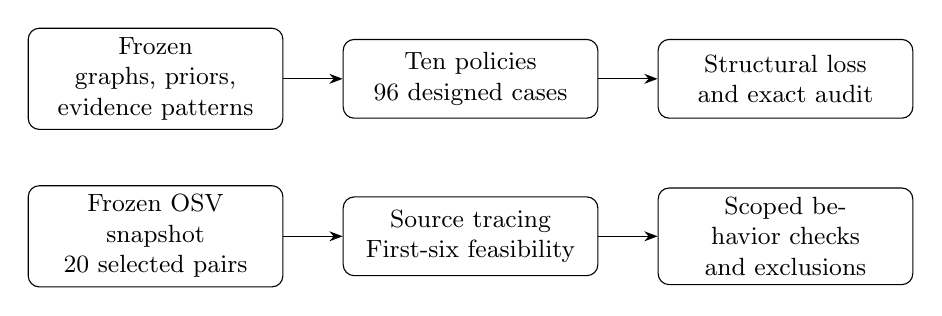
\begin{tikzpicture}[>=Stealth,box/.style={draw,rounded corners,align=center,text width=3cm,minimum height=1cm,font=\small}]
\node[box] (g) at (0,1) {Frozen graphs, priors,\\evidence patterns};
\node[box] (p) at (4,1) {Ten policies\\96 designed cases};
\node[box] (l) at (8,1) {Structural loss\\and exact audit};
\node[box] (a) at (0,-1) {Frozen OSV snapshot\\20 selected pairs};
\node[box] (s) at (4,-1) {Source tracing\\First-six feasibility};
\node[box] (b) at (8,-1) {Scoped behavior checks\\and exclusions};
\draw[->] (g)--(p); \draw[->] (p)--(l);
\draw[->] (a)--(s); \draw[->] (s)--(b);
\end{tikzpicture}
\caption{Two separate evidence streams. Public artifacts support the feasibility audit; they do not calibrate the designed graph probabilities or losses.}
\Description{The upper lane connects synthetic inputs to policy evaluation and exact scoring. The lower lane connects a public snapshot to source tracing and scoped behavioral checks. The lanes are separate.}
\end{figure}
\subsection{Frozen synthetic grid}
The validation specification was committed and hash-sealed before collection. Three four-gate graph families are crossed with two priors, eight evidence patterns, and two query costs: $3\times2\times8\times2=96$ cases. Ten policy rows per case give 960 evaluations. These are designed cases, not a random sample of networks. Earlier two- and three-gate calculations were development examples and are not added to the validation denominator.

The independent prior assigns probability $1/16$ to each state. The shared-cause mixture assigns half its mass to that uniform distribution and another quarter each to states $0000$ and $1111$. Gate marginals are one half in both priors before observing reports, allowing dependence to vary without changing those initial marginals. Total budget is 1.5, query accuracy is 0.9, and query costs are 0.25 and 0.75. No parameters are estimated from public advisories.

\begin{table}[t]
\caption{Validation graphs. An edge is written source--destination:gate. Targets have specified model weights.}
\label{tab:graphs}
\begin{tabularx}{\linewidth}{lXl}
\toprule
Graph & Directed edges & Targets \\
\midrule
Diamond & $s\!\to\!l:0$, $s\!\to\!r:1$, $l\!\to\!t:2$, $r\!\to\!t:3$ & $t:10$ \\
Shared bridge & $s\!\to\!m:0$, $m\!\to\!a:1$, $m\!\to\!b:2$, $a\!\to\!b:3$ & $a:10,b:8$ \\
Bypass cycle & $s\!\to\!a:0$, $a\!\to\!b:1$, $b\!\to\!a:2$, $s\!\to\!b:3$, $b\!\to\!t:2$ & $a:4,t:10$ \\
\bottomrule
\end{tabularx}
\end{table}

\begin{figure}[t]
\centering
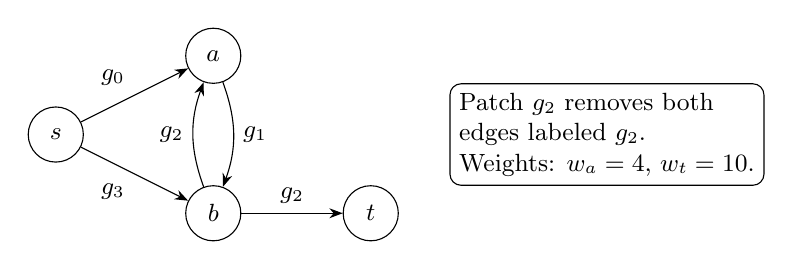
\begin{tikzpicture}[>=Stealth, every node/.style={font=\small}, vertex/.style={circle,draw,minimum size=7mm}]
\node[vertex] (s) at (0,0) {$s$};
\node[vertex] (a) at (2,1) {$a$};
\node[vertex] (b) at (2,-1) {$b$};
\node[vertex] (t) at (4,-1) {$t$};
\draw[->] (s)--node[above left] {$g_0$}(a);
\draw[->] (s)--node[below left] {$g_3$}(b);
\draw[->] (a) to[bend left=20] node[right] {$g_1$} (b);
\draw[->] (b) to[bend left=20] node[left] {$g_2$} (a);
\draw[->] (b)--node[above] {$g_2$}(t);
\node[draw,rounded corners,align=left] at (7,0) {Patch $g_2$ removes both\\edges labeled $g_2$.\\Weights: $w_a=4$, $w_t=10$.};
\end{tikzpicture}
\caption{The bypass-cycle graph used in the dependence counterexamples. The same latent gate controls two edges; graph dependence is distinct from copied-report dependence.}
\Description{Entry s connects to a through gate zero and b through gate three. Gate one connects a to b. Gate two connects b to a and b to target t.}
\end{figure}

All evidence patterns concern gate 2. The base positive report has accuracy 0.8. Patterns are one report; four correctly grouped copies; four copies falsely split into separate sources; independent positive and negative reports; those conflicting independent reports falsely merged; a correctly reported flip probability of 0.4; the same true flip probability reported as zero; and false splitting combined with unreported staleness. Table~\ref{tab:evidence} specifies the corresponding evaluator relationships.

\begin{table}[t]
\caption{Designed evidence patterns. True source and true flip are evaluator-only fields.}
\label{tab:evidence}
\begin{tabularx}{\linewidth}{lX}
\toprule
Pattern & Construction \\
\midrule
Single & One positive source, no flip. \\
Copies correct & Four copies of one positive source, correctly grouped. \\
Copies split & Same underlying report, four distinct reported source labels. \\
Independent conflict & Separate positive and negative sources, correctly labeled. \\
False merge conflict & Independent conflicting reports assigned one label. \\
Stale correct & One positive source, true and reported flip 0.4. \\
Stale underestimated & One positive source, true flip 0.4, reported flip zero. \\
Split and stale & Four copies, false splitting, true flip 0.4, reported flip zero. \\
\bottomrule
\end{tabularx}
\end{table}

The primary endpoint is lineage-and-age VOI loss minus its immediate counterpart, paired within each case. Counts use tolerance $10^{-9}$. Secondary outputs include every policy's loss, spend, query selection, dropped conflicting groups, and oracle regret. Equal weighting describes this finite grid only. Cases share graphs and observations, so we report no population confidence intervals or hypothesis-test $p$-values.

\subsection{Execution and independent arithmetic audit}
The frozen validation completed on ASA-X under PBS job 97288.asax-pbs1 using Python 3.9.21. All 96 cases completed with zero execution failures. The saved run identifies source revision and hashes. Post hoc analysis verifies completeness, source integrity, branch budgets, saved summaries, and regret arithmetic.

A separate standard-library implementation then reconstructs the evaluator distribution using rational numbers and computes reachability by graph traversal. It scores the saved decisions rather than rerunning or tuning policy selection. Across all 960 rows, expected loss and spend agree within $10^{-9}$; maximum loss discrepancy is approximately $1.33\times10^{-15}$. This is an independent implementation check by the same research workflow, not an external replication. It cannot establish that the model assumptions represent a real network.

\subsection{Public selection and source audit}
The public study uses a single current official OSV PyPI export~\cite{osv}. Eligible records have GHSA identifiers, published dates during 2023--2025, an affected PyPI package, and an explicit fixed event. Withdrawn records and the prior Requests development advisory are excluded. Advisory IDs and normalized package names determine lexicographic order. The first 20 unique pairs form a deterministic convenience sample; difficult cases are not replaced.

The snapshot contains 26,104 records. Screening identifies 1,521 eligible records and 1,600 unique eligible pairs; 24,583 records are excluded, with overlapping exclusion reasons. No parser failures occurred. A hash identifies the archive and a complete screening ledger accounts for records. The first six selected pairs define the behavioral-feasibility subset. Source attribution is traced through explicit fields, not similarity of wording. Linked GitHub records are pinned to one repository revision and compared on identifiers and structured ranges. Shared aliases are recorded separately from source copying.

The public protocol records two feasibility expectations: that some selected records permit explicit source tracing, and that some selected version pairs permit repeatable isolated checks. These are descriptive expectations, not novel scientific laws or statistically powered hypotheses. Unknowns and unsupported fixtures remain in the denominator.

\subsection{Behavioral feasibility}
For each selected pair, the protocol chooses the lowest qualifying stable fixed release and the greatest preceding stable release marked affected in the same interval. A case without such a stable fixed event remains excluded. Each executable check has a committed pre-execution addendum defining versions, dependencies, observable property, benign control, resource limits, and outcome rules. Original probes use public synthetic fixtures only. Advisory-informed design is disclosed and does not constitute independent vulnerability discovery.

Dependency acquisition and source builds run in restricted disposable containers. Behavior containers have no network, read-only roots and artifact mounts, dropped capabilities, no-new-privileges, bounded resources, and disposable temporary storage. Probes do not send attacks to external systems. Three repetitions assess repeatability; they are not three independent vulnerabilities. Installation failures, import failures, timeouts, and parser issues are preserved separately from valid behavioral observations.

\section{Results}\label{sec:results}
\subsection{Verification gains and their attribution}
The primary policy improves expected loss in 27 of 96 cases, ties in 69, and worsens in none. The results are heterogeneous by graph and query affordability (Table~\ref{tab:primary}). All 32 shared-bridge cases tie because gate 0 is an affordable universal cut. All 48 expensive-query cases tie because querying prevents every nonempty patch set. These groups overlap and must not be added as independent explanations.

\begin{table}[t]
\caption{Primary paired outcome counts, VOI versus immediate action for lineage-and-age. Subgroups overlap.}
\label{tab:primary}
\begin{tabular}{lrrrr}
\toprule Condition & Cases & Lower loss & Tie & Higher loss \\
\midrule
All &96&27&69&0\\
Query cost 0.25 &48&27&21&0\\
Query cost 0.75 &48&0&48&0\\
Independent prior &48&16&32&0\\
Shared-cause mixture &48&11&37&0\\
Diamond &32&16&16&0\\
Shared bridge &32&0&32&0\\
Bypass cycle &32&11&21&0\\
\bottomrule
\end{tabular}
\end{table}

Every immediate family has finite-grid mean loss 1.865833. Naive and deduplicated VOI both have mean loss 1.701417, compared with 1.701167 for lineage-and-age and 1.700667 for the privileged model. Thus the gain against immediate patching is much larger than the incremental provenance/age gain. The latter is 0.00025 in mean loss, arising from one material case difference of 0.024 divided by 96. It occurs in the shared-cause bypass graph with correctly reported staleness and cheap querying, where loss changes from 2.12 to 2.096. Deduplication alone does not improve loss over naive verification on this grid.

\begin{table}[t]
\caption{All-policy descriptive aggregates. Mean loss and spend weight each designed case equally. I denotes immediate action and V denotes optional verification.}
\label{tab:policies}
\begin{tabular}{lrrrr}
\toprule Policy & Mean loss & Mean spend & Mean oracle regret & Queries \\
\midrule
Naive I &1.865833&1.000000&0.767813&0\\
Naive V &1.701417&1.075521&0.603396&29\\
Deduplicated I &1.865833&1.000000&0.767813&0\\
Deduplicated V &1.701417&1.072917&0.603396&28\\
Lineage/age I &1.865833&1.000000&0.767813&0\\
Lineage/age V &1.701167&1.075521&0.603146&29\\
Factorized I &1.865833&1.000000&0.767813&0\\
Factorized V &1.704667&1.078125&0.606646&30\\
Privileged I &1.865833&1.000000&0.767813&0\\
Privileged V &1.700667&1.075521&0.602646&29\\
\bottomrule
\end{tabular}
\end{table}

\subsection{A harmful dependence approximation}
Two shared-cause bypass cases, with single evidence and correctly grouped copies at query cost 0.25, show harm from factorization. The factorized VOI policy queries gate 3 and patches gate 0 or gate 2 depending on the answer. Scoring this decision under the joint evaluator distribution gives loss 2.78. Immediate patching of gate 2 gives 2.60, so verification increases expected loss by 0.18. The joint lineage-and-age policy chooses immediate action. The two cases differ in report representation but share the underlying observation, and are not independent empirical replications.

The result is consistent with the analytical optional-verification property: the factorized planner optimizes its own approximate belief, while evaluation uses the joint model. It does not demonstrate that additional information itself is harmful under a correctly specified model. Nor does it estimate how frequently factorization harms deployed systems.

\subsection{Numerical ties and evidence conflicts}
In two false-splitting cases on the shared-cause bypass graph, lineage-and-age queries gate 0 but patches gate 2 for either answer. Expected loss ties immediate action within tolerance, while spend increases from 1 to 1.25. Raw floating-point comparison of algebraically equal risks explains these redundant queries. One naive-policy case also has a redundant query that grouping avoids without changing loss. Outcome-count tolerance and planner tie handling are different mechanisms.

Grouped policies discard conflicting reported groups in 12 cases. This behavior is an implementation consequence of the conflict rule, not evidence that discarding reports improves decisions. Incorrect source labels remain a limitation. We neither fix numerical ties nor retune the conflict rule inside the sealed experiment.

\subsection{Public provenance}
All 20 selected pairs explicitly attribute a GitHub Advisory Database source. Every source retrieval succeeds at pinned revision \texttt{963f4b6} (full identity in the artifact), and all 20 identifier and structured-range comparisons match. No selected entries share aliases with one another. This does not establish independent observations, and the 20/20 attribution result is expected from selecting GHSA records. It is not an estimate of ecosystem-wide dependence.

All 20 source modified timestamps differ from the corresponding OSV timestamps. Processing timestamps are not vulnerability-truth clocks: these differences alone establish neither staleness nor changed affectedness. Likewise, agreement between copied database records is not an independent behavioral observation. The source audit motivates provenance-aware interpretation but supplies no calibrated query accuracy or graph-state probabilities.

\subsection{Public behavioral results}
\label{sec:public-results}
Four of the six selected cases establish the predefined narrow distinction, one is excluded by the stable-fixed-release rule, and one is unsupported within the fixture restrictions (Table~\ref{tab:public}). There are 21 successful final container runs: six each for Langroid, pretalx, and Scrapy, plus three certifi runs that each compare both bundles. These counts describe feasibility in the selected subset, not a population success rate.

\begin{table}[t]
\caption{Complete first-six case dispositions. No replacements were made. Versions are affected/fixed candidates from the frozen advisory selection.}
\label{tab:public}
\begin{tabularx}{\linewidth}{llX}
\toprule Package & Versions & Verified scope or disposition \\
\midrule
InvokeAI & Only fixed event 5.3.0rc1 & Excluded: no qualifying stable fixed event. \\
Langroid & 0.53.14 / 0.53.15 & Actual compute\_from\_docs method accepts benign DataFrame count in both; harmless len(df) changes from returning 2 to a sanitizer error. Malformed-input controls also pass. \\
pretalx & 2.3.1 / 2.3.2 & Actual dump\_content writes a traversal path outside the export directory, within the disposable fixture, only in the old version. The fixed version raises CommandError. Ordinary export succeeds in both. \\
Scrapy & 2.11.1 / 2.11.2 & Both redirect middleware paths return Requests for HTTPS controls in both versions; file-URI redirects produce Requests only in the old version. No returned request is followed. \\
WordOps & 3.20.0 / 3.21.0 & Dependencies build, but the real affected path performs system provisioning and uses hard-coded system paths. Unsupported under the frozen fixture; no race claim reproduced. \\
certifi & 2024.6.2 / 2024.7.4 & Fresh SSL contexts loading each original bundle include the specified GLOBALTRUST 2020 fingerprint only in the older bundle. Empty-context and common-certificate controls pass. \\
\bottomrule
\end{tabularx}
\end{table}

All predefined observations and controls pass in all three repetitions for each executable pair. The Langroid invocation calls the real installed method with an unused self argument and real Document objects, without constructing an embedding service. The pretalx invocation initializes the installed Django application and calls its export function with a constant-byte getter, without serving requests or querying a populated database. Certifi checks load the original certificate bundle through Python's SSL context rather than calling certifi's API. Each distinction is advisory-informed and restricted to the stated path~\cite{advisories}.

Preparation failures are part of the result. Scrapy first failed because its temporary filesystem disallowed executable virtual-environment tools, then because a newly resolved w3lib was incompatible. Versioned amendments enabled execution on disposable temporary storage and pinned w3lib 2.2.1. Langroid first failed when import required an uncached tokenizer file, then because the initial Document fixture lacked required metadata. Subsequent runs use hash-verified public tokenizer data and corrected fixture construction. Across these series, 24 failed container runs are retained. Additional wheel-only and source-build failures are separately recorded and are not counted as these 24 runs. Pretalx source builds on Python 3.11 failed for lack of a C compiler; Python 3.9 preparation succeeded.

The pretalx application prints a startup banner before the JSON observation. Its original runner accordingly marked a JSON parse error despite successful execution. A separate analysis extracts the single complete JSON record from each preserved stdout file, checks the version and observations, and retains the original parse-error flag. No behavior is rerun or changed to resolve this reporting issue.

Shared dependency artifacts are identical within the final Langroid and pretalx pairs. Independently built Langroid halo and wget wheel archives initially differed in hashes but had identical member bytes; the final environments use one artifact for each shared filename. Scrapy's fixed environment adds defusedxml, so it is not a sole-code-change comparison. The observed package distinction is conditional on these environments.

\begin{table}[t]
\caption{Descriptive runtime measurements for successful final runs. Probe timing includes imports as implemented. RSS is peak process memory, not whole-container memory. Concurrent preparation and run activity was not controlled as a performance benchmark.}
\label{tab:runtime}
\begin{tabular}{lrrrr}
\toprule Package & Runs & Probe median (s) & Probe range (s) & Max RSS (KiB) \\
\midrule
Langroid &6&2.793&2.447--8.036&213064\\
pretalx &6&1.855&1.407--4.699&69616\\
Scrapy &6&0.617&0.565--0.707&57744\\
certifi &3&0.041&0.040--0.053&23140\\
\bottomrule
\end{tabular}
\end{table}

Median setup-plus-container elapsed times are 87.508, 36.648, 17.321, and 1.109 seconds respectively. Subtracting probe time does not isolate installation time; it also includes container and teardown overhead. These timings are environment receipts, not operational patch costs. The two-hour engineering cap was not exhausted for WordOps; its disposition follows the unsupported-fixture rule, not a fabricated timeout.

\section{Discussion}
\subsection{Decision relevance precedes evidence volume}
The benchmark separates three questions that can otherwise be conflated: whether a report is more trustworthy, whether a query changes the selected patch, and whether that changed patch reduces loss under the evaluator distribution. More reports need not provide more information when they copy one event. Better information need not change an already optimal universal cut. A changed action need not improve consequences when joint dependence is misrepresented.

The largest observed difference is between optional verification and immediate action, not between naive and provenance-aware verification. Consequently, an evaluation containing only an immediate baseline would overstate the mechanism supported by these data. Including ordinary VOI, grouping without age correction, and a privileged-model comparator reveals how little additional benefit is attributable to provenance/age handling in this grid.

\subsection{The budget boundary is structural}
The expensive-query result is often tempting to describe as evidence that verification is too costly. A more precise explanation is that the selected cost crosses a discrete action-feasibility boundary. With budget 1.5 and unit patches, the two query prices change whether any patch is possible. A deployment could have fractional interventions, different costs, sequential learning, or future reuse of information. Those settings would require a different analysis. The present result establishes a mechanism and a negative control, not a general economic recommendation.

\subsection{Public evidence does not close the calibration gap}
Executable package checks provide a channel beyond database agreement, but their scope must match their observable property. Redirect middleware behavior is not proof of downloaded file access. Trust-anchor removal is not a complete TLS safety assessment. An expression-sanitization check is not a guarantee against arbitrary agent compromise. An export function fixture does not reproduce a production deployment. These distinctions prevent narrow successful checks from being promoted into universal fixed-version labels.

The public audit and synthetic experiment therefore remain separate evidence streams. Joining them would require measured observation accuracy, deployment topology, intervention effects, and costs under an explicit sampling design. Converting severity scores, record counts, or timestamps into those parameters would invent calibration. The scoped go/no-go decision is to publish the bounded benchmark and feasibility characterization, while declining an operational superiority claim.

\section{Threats to Validity}
\paragraph{Construct validity.} Weighted reachability omits attacker behavior, patch disruption, exploit prerequisites beyond the gates, and time. Target weights and probability parameters are designed. Source labels represent measurement-event grouping in the model; a shared advisory publisher is not automatically the same object. The age mechanism is a binary flip model. None of these constructs has been calibrated with the public package sample.

\paragraph{Internal validity.} Exact enumeration avoids Monte Carlo sampling error, but code and specification errors remain possible. Sealed inputs, unit tests, invariant checks, retained decisions, and independent rational scoring reduce these risks. The rational audit reuses the stated specification and thus cannot detect a flawed scientific assumption. Frozen floating-point tie behavior remains visible. Setup amendments were committed before corrected runs; the failed runs are not removed from the record.

\paragraph{External validity.} Three four-gate graphs do not represent enterprise networks. The 96 crossed cases reuse graphs and evidence patterns. The 20 public pairs are lexicographically selected GHSA/PyPI examples, not a random sample. Only the first six are assessed for behavioral feasibility. Package versions, Python runtimes, and transitive dependencies limit transportability. Multiple repetitions establish repeatability on the tested environment, not generalization across operating systems or independent vulnerabilities.

\paragraph{Comparison validity.} The benchmark does not reproduce dynamic security games, CAPG-v2, or a production remediation product. Their endpoints and assumptions differ. The privileged model and perfect-state oracle are diagnostic comparators, not accessible deployed solutions. The observed tiny provenance advantage should not be reported as broad superiority, and the constructed dependence harms should not be interpreted as prevalence estimates.

\paragraph{Reproducibility limits.} The original snapshot and downloaded third-party artifacts are retained outside Git, with identifiers and hashes in the repository. Mutable public endpoints may later change or remove artifacts. Hashes detect changes but do not guarantee future availability or establish external preregistration. Source builds can produce byte-different ZIP containers; comparison environments use identical shared wheels where possible. Reconstructing an environment may require the retained original artifacts, not merely current package names.

\section{Artifacts, Ethics, and Research Transparency}
The repository at \url{https://github.com/ezekielologunde/attack-graph-evidence-quality} contains model code, frozen specifications, case-level results, screening and provenance ledgers, probe code, environment locks, failed-run logs, and verification scripts. Public packages and advisory records are used as research artifacts. No private participant data or live external targets are involved. Original work is intentionally unlicensed pending the author's reuse decision; third-party rights and notices remain separate.

The reproducibility guide distinguishes replay of saved arithmetic from reacquisition, rebuilding dependencies, and rerunning isolated package behavior. The latter can be slower and depends on public artifact availability. Synthetic validation used ASA-X; the public function checks ran locally in Docker. Neither a GPU experiment nor enterprise-scale performance measurement is claimed.

Generative AI through OpenAI Codex contributed to code development, literature triage, analysis, and manuscript drafting. It is not an author. The manuscript is supplied for human author review; no claim is made that author approval, journal acceptance, peer review, or submission has occurred. The author is an independent researcher; the email domain does not imply institutional affiliation. No corresponding-author designation is made. The destination journal remains to be selected.

\section{Conclusion}
In this finite structural-remediation benchmark, verification is useful when it can change an affordable intervention and when the planning model represents decision-relevant dependence adequately. Universal cuts and residual-budget constraints explain major no-benefit regions. An independence approximation yields two explicit harmful-query examples, while provenance/age handling adds only a small mean-loss improvement over naive VOI. The public audit establishes traceable source relationships and bounded behavioral feasibility, without supplying operational calibration. The released cases, negative controls, exact arithmetic audit, and preserved failures support a reproducible methods study. They do not support a new-algorithm claim or demonstrated improvement to real-world remediation.

\begin{thebibliography}{9}
\bibitem{nguyen} Hoang Hai Nguyen, Kartik Palani, and David M. Nicol. 2017. An Approach to Incorporating Uncertainty in Network Security Analysis. In \emph{HoTSoS}. \url{https://doi.org/10.1145/3055305.3055308}.
\bibitem{krause} Andreas Krause and Carlos Guestrin. 2009. Optimal Value of Information in Graphical Models. \emph{Journal of Artificial Intelligence Research} 35, 557--591. Author manuscript: \url{https://arxiv.org/abs/1401.3474}.
\bibitem{dong} Xin Luna Dong, Laure Berti-Equille, and Divesh Srivastava. 2009. Integrating Conflicting Data: The Role of Source Dependence. \emph{Proceedings of the VLDB Endowment}. \url{https://www.vldb.org/pvldb/vol2/vldb09-pvldb47.pdf}.
\bibitem{khakpour} Narges Khakpour and David Parker. 2022. Partially-Observable Security Games for Automating Attack-Defense Analysis. arXiv:2211.01508v1. \url{https://arxiv.org/abs/2211.01508}.
\bibitem{cygate} Yuning Jiang, Nay Oo, Qiaoran Meng, Lu Lin, Dusit Niyato, Zehui Xiong, Hoon Wei Lim, and Biplab Sikdar. 2025. CyGATE: Game-Theoretic Cyber Attack-Defense Engine for Patch Strategy Optimization. arXiv:2508.00478v1. \url{https://arxiv.org/abs/2508.00478}.
\bibitem{capg} Noufal Issa, Damas Gruska, and Loubna Ali. 2026. CAPG-v2: Impact-Weighted, Multi-Path Vulnerability Prioritization over CVE-Centric Attack-Position Graphs. In \emph{SECRYPT}, Vol. 2, 1089--1096. \url{https://doi.org/10.5220/0015064100004103}.
\bibitem{osv} OSV. Data Sources and Exports. Retrieved 7 October 2026. \url{https://google.github.io/osv.dev/data/}.
\bibitem{advisories} GitHub Advisory Database. Selected records GHSA-227r-w5j2-6243, GHSA-22c2-9gwg-mj59, GHSA-23fx-92m6-4f2g, GHSA-23j4-mw76-5v7h, GHSA-23qq-p4gq-gc2g, and GHSA-248v-346w-9cwc. Pinned source revision 963f4b691a2736e0bb288f5f855915bf7ffd3c3e, retrieved 7 October 2026. \url{https://github.com/github/advisory-database/tree/963f4b691a2736e0bb288f5f855915bf7ffd3c3e}. Exact record and patch links are retained in the research artifact.
\end{thebibliography}
\end{document}
